\documentclass[12pt, a4paper, oneside]{article}

\usepackage[T1]{fontenc}
\usepackage[british]{babel}
\usepackage{lmodern}
\usepackage{graphicx}
\usepackage{hyperref}


\renewcommand{\familydefault}{\sfdefault}

\author{}
\date{}

\title{CM10227 Getting Started}

\begin{document}
\maketitle

This is a short guide to preparing, checking and submitting coursework for CM10227.
In order to satisfy the coursework requirements, you will need to write code, check that it compiles and runs on \href{http://www.bath.ac.uk/guides/connecting-to-linux-bath/}{linux.bath} and submit the original source code (.c files) to Moodle.

\section{Writing Code}

\subsection{Using an online IDE}
Perhaps the easiest way to begin programming in C, is to use an online IDE.
This will simplify the process of compiling and running code as you get used to programming.
One option is \url{https://www.codechef.com/ide}.
You should download any code you wish to submit, and later test it on \href{http://www.bath.ac.uk/guides/connecting-to-linux-bath/}{linux.bath} prior to submission.

 \subsection{Using Windows and Notepad++}
 If you wish to code offline (our recommended approach once you are familiar with each of the steps in this document), you must use a (plain) text editor: Microsoft Word is \textbf{not} suitable for this task.
 One option is to use Notepad++.
 You can download a standalone version here: \url{https://notepad-plus-plus.org/repository/6.x/6.8.3/npp.6.8.3.bin.zip}.
 Make sure you save your source file with a ``.c'' extension; once Notepad++ recognises that you're writing C code, it will start highlighting the syntax accordingly.

\subsection{Using Linux (\href{http://www.bath.ac.uk/guides/connecting-to-linux-bath/}{linux.bath}) to write and edit code}
You can also use a Linux text editor at the University to write your code on \href{http://www.bath.ac.uk/guides/connecting-to-linux-bath/}{linux.bath}. One example is gedit, though others exist e.g. emacs, vim, nano, ed.
Once you have logged in to \href{http://www.bath.ac.uk/guides/connecting-to-linux-bath/}{linux.bath} (see the next section), you can use gedit by typing "gedit\&" at the command prompt.
\begin{figure}[h!]
  \caption{The choice of text editor is a contentious topic: https://xkcd.com/378/}
  \centering
    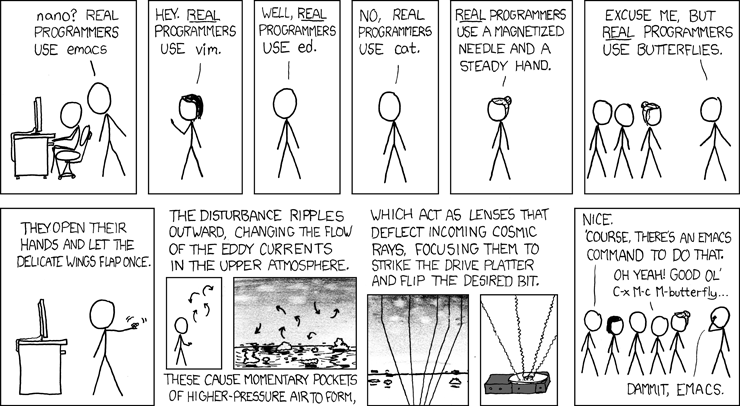
\includegraphics[width=\textwidth]{real_programmers.png}
\end{figure}

\section{Using \href{http://www.bath.ac.uk/guides/connecting-to-linux-bath/}{linux.bath} to compile and run code}
\href{http://www.bath.ac.uk/guides/connecting-to-linux-bath/}{linux.bath} is set of three servers maintained by the University, running Ubuntu 14.04.
You can access these using Secure SHell (SSH).
This provides a command-line interface (BaSH) and the ability to access GUI applications.

From a BUCS computer, or \href{http://www.bath.ac.uk/bucs/tools/windowsterminalservices/}{Unidesk}, you can access linux.bath by clicking ``start'', typing in linux.bath and selecting the shortcut.
This will start an SSH session (the first time you access, accept the certificate).
If you wish to access \href{http://www.bath.ac.uk/guides/connecting-to-linux-bath/}{linux.bath} from your own machine, please refer to the online \href{http://www.bath.ac.uk/bucs/networking/ssh.html}{instructions}.

The current working directory will be your ``home'' directory, which is conveniently the same as the ``H:'' drive on the BUCS computer.
\textit{View ``H:''  on the BUCS computer (i.e. in ``Computer'' on the desktop), then type in ``ls'' to see that these are indeed the same.}
\textit{To get back here at any time, type in ``cd \textasciitilde''.}

Once you have written your code (using one of the methods above) and copied it to a location you can reach on linux.bath (the tutors will help with this), you can compile using gcc. It is safest to use gcc as follows, changing "HelloWorld" for your source file:
\textit{gcc -o HelloWorld -Wall HelloWorld.c -lm} (Without the ``-o'' flag, gcc will produce a file called a.out, and the ``-Wall'' turns on helpful warnings.)

\textit{Run the program by typing ``./HelloWorld''.} The ``./'' is needed as it indicates that the program in the current directory must be run: by default this is not in the search path.

You can now begin programming.


\end{document}
